
\section{Design}
\label{cp6:design}


% To understand how a tool embedding a semantic-based technique might impact a developer's work,
% we are guided by three main factors.


To design our experiment, we consider three main aspects that assist us examine how a tool that embeds a semantic-based technique might impact a developer's work, namely \textit{prominence}, \textit{correctness}, and \textit{usefulness}.




\begin{description}[leftmargin=\parindent, font=\normalfont\itshape]
    
    \item[Prominence.] To be helpful, a tool must direct a developer's attention to text that assist them complete a task~\cite{Robillard2015}.
    Hence, our experiment must have a means to assess whether the text automatically identified by the tool is similar to text considered by humans as relevant to the task at hand. 


    \item[Correctness.] If the text identified by the tool is not similar to the text identified by humans,
    there is a chance that the tool directed a participant to the wrong information, or that 
    the tool actually found complementary information that humans missed, which might impact the correctness of a task. 
    Therefore, evaluation should also compare the correctness of solutions submitted by participants who perform a task using such a tool against a control group.

    \item[Usefulness.] Regardless of how correct participants' solutions are, there is a chance that the text shown by the tool is not useful, either because it is not relevant for the task at hand or because it is unsurprising, i.e., the information is ``common-knowledge'' to most developers~\cite{cwalina2008, Robillard2015}. Hence, a successful evaluation must
    examine the usefulness of the text identified by the tool. 
    
\end{description}









% To show how this experiment allows such a investigation, we begin by detailing
% experimental procedures (Sections~\ref{cp6:design} to~\ref{cp6:procedures}).
% Then, we discuss how we analyze the data obtained from the experiment by:


% \begin{itemize}
%     \item assessing the correctness of the tasks performed \textit{with} or \textit{without} tool support (Section~\ref{cp6:correctness});
%     \item comparing  the text that participants deemed relevant to the text automatically identified
%     and shown in the tool-assisted task (Section~\ref{cp6:comparison}), and;
%     \item discussing the usefulness of the automatically identified text according to the feedback provided by the participants (Section~\ref{cp6:usefulness}).
% \end{itemize}
 





% \begin{figure}
% \centering
% 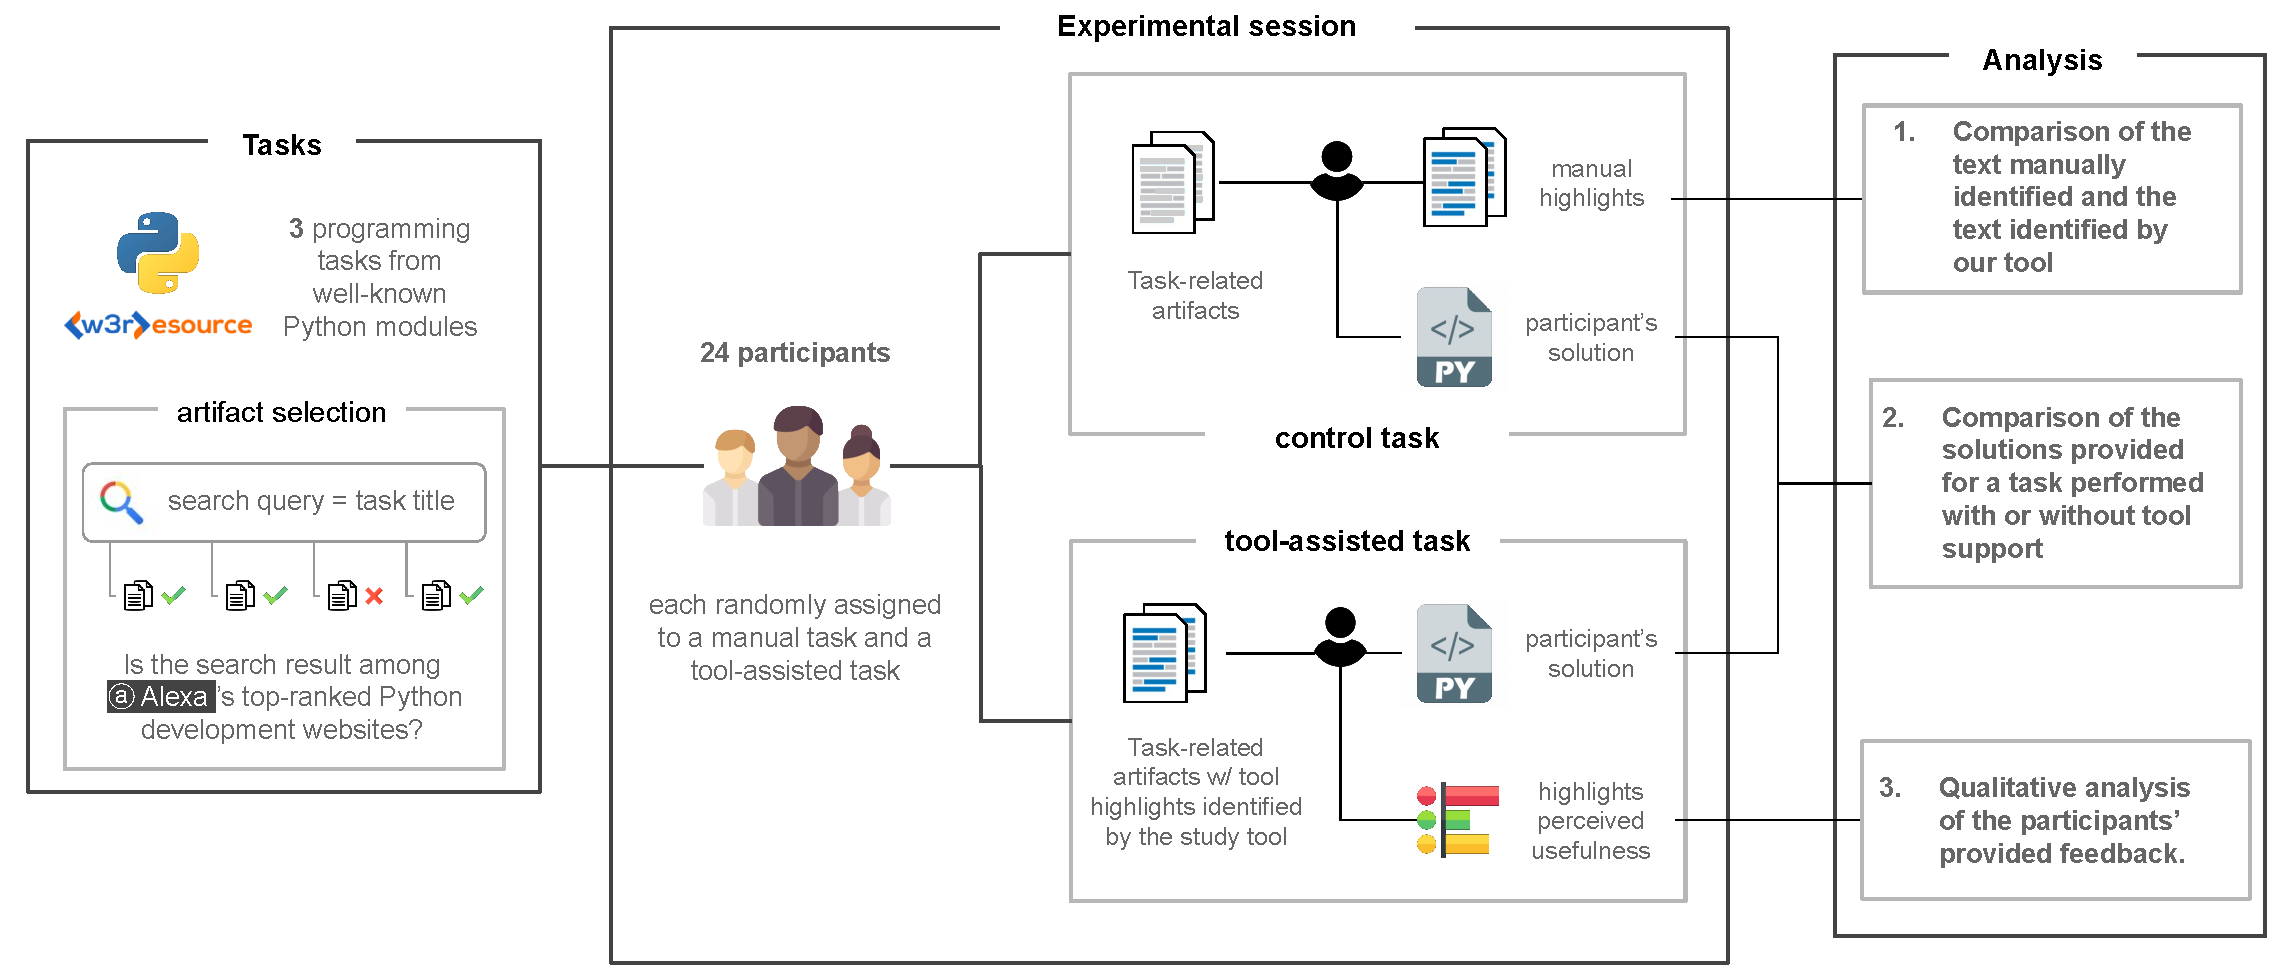
\includegraphics[width=1.05\textwidth]{cp6/tool-experiment-pipeline.pdf}
% \caption{Summary of experimental procedures}
% \label{fig:tool-experiment-procedures}
% \end{figure}





The experiment that we describe in Figure~\ref{fig:tool-experiment-procedures} is designed around these driving factors.  
Each participant attempted two randomly assigned Python programming tasks on their own time and computer\footnote{Literature define this as an \textit{offline} experiment~\cite{wohlin2012, DeLucia2012}}.
In a first task, i.e., \textit{manual task}, a participant indicated 
what text they deemed relevant to the task at hand while 
they consulted a curated list of artifacts that could assist them in writing a solution for that task.
In a second task, i.e., \textit{tool-assisted task},
participants wrote their solution consulting a similar list of curated artifacts, but
assisted by a tool that highlighted the text identified as potentially relevant to their task; for this task, we also gathered feedback on the usefulness of the highlights shown.

 

With this experiment we evaluate different factors that can help us answer whether 
a tool embedding a semantic-based technique helps developers complete a software task. 
